% !TeX root = main.tex
\section*{Lithographic system}
The basic working of optical contact lithography is illustrated in figure \ref{fig:contact-litho}. Light emitted from a source is collimated using a condenser lens (or an array of lenses). The collimated light travels through the transparent parts of the mask and illuminates the resist areas directly below these areas. 
\begin{figure}[H]
	\centering
	\resizebox{0.7\linewidth}{!}{% !TeX root = main.tex
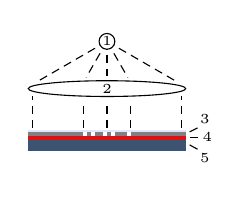
\begin{tikzpicture}
    % Sample
    \fill[fill={rgb:red,66;green,91;blue,121}] (-1,-1.24) rectangle (1,-1.39);
    \draw (1.05,-1.315) to node [below right = -.4 mm] {\tiny $5$} (1.15,-1.37);
    % Resist
    \fill[fill={rgb:red,198;green,15;blue,15}] (-1,-1.20) rectangle (1,-1.24);
    \draw (1.05,-1.22) to node [right = -.1 mm] {\tiny $4$} (1.15,-1.22);
    % Mask
    \foreach \x/\y in {0/.7,.75/.8,.85/0.95,1/1.05,1.1/1.25,1.3/2}
        \fill[fill=gray] (\x-1,-1.15) rectangle (\y-1,-1.20);
    \draw (1.05,-1.15) to node [above right = -.4 mm] {\tiny $3$} (1.15,-1.10);
    % Glass plate
    \fill[fill=blue!10] (-1,-1.12) rectangle (1,-1.15);
    % Lens
    \draw (0,-.6) ellipse [x radius=1, y radius=.1] node {\tiny $2$};
    % Light rays
    \foreach \angle/\r in {210/1,240/.53,270/.44,300/.53,330/1}
        \draw[densely dashed] (0,0) -- (\angle:\r);
    \foreach \x/\y in {-.95/.7,-.3/.75,0/.75,.3/.75,.95/.7}
        \draw[densely dashed] (\x,-1.1) -- (\x,-\y);
    % Light source
    \draw[fill=white] (0,0) ellipse [x radius=.1, y radius=.1] node {\tiny $1$};
\end{tikzpicture}
}
	\caption{Simplified working of contact lithography, where 1. light source, 2. condenser lens(es), 3. glass/quarts plate with mask, 4. photographic resist, 5. substrate. Dashed lines indicate light paths.}
	\label{fig:contact-litho}
\end{figure} For this experiment a MJB-3 from Karl Suss Microtec with a mercury-vapor lamp was used. However, this particular model is designed for deep ultraviolet (DUV) while the used resist is designed for exposure to the I-line and H-line (365.4~nm and 404.7~nm respectively) of the lamp or near ultraviolet (NUV). To prevent the DUV light from exposing the resist and damaging it, the mask is clamped to a glass plate which blocks light with $\lambda \lesssim 300$~nm.

\todo[inline]{Piece about the mask, maybe including some pictures} 

\section*{Substrate and resist}
Patterns were written on a series of square cut silicon substrates of approximately 15 mm by 15 mm. For both the negative and positive tone samples, AZ~5214E\footnote{AZ~5214E is a high resoluation image reversal resist produced by MicroChemicals} is used as photoresist. Since the optics of the MJB-3 is designed for DUV light, much intensity of the NUV is absorbed. Thus the exposure times of standard recipes designed by the Kavli Nanolab facility are not sufficient. The recipes are modified to accommodate the decrease in light intensity. Some initial guessing was needed and different exposure times are  investigated.

\begin{figure*}[!b]
    \centering
    \begin{subfigure}[t]{0.3\linewidth}
        \centering
        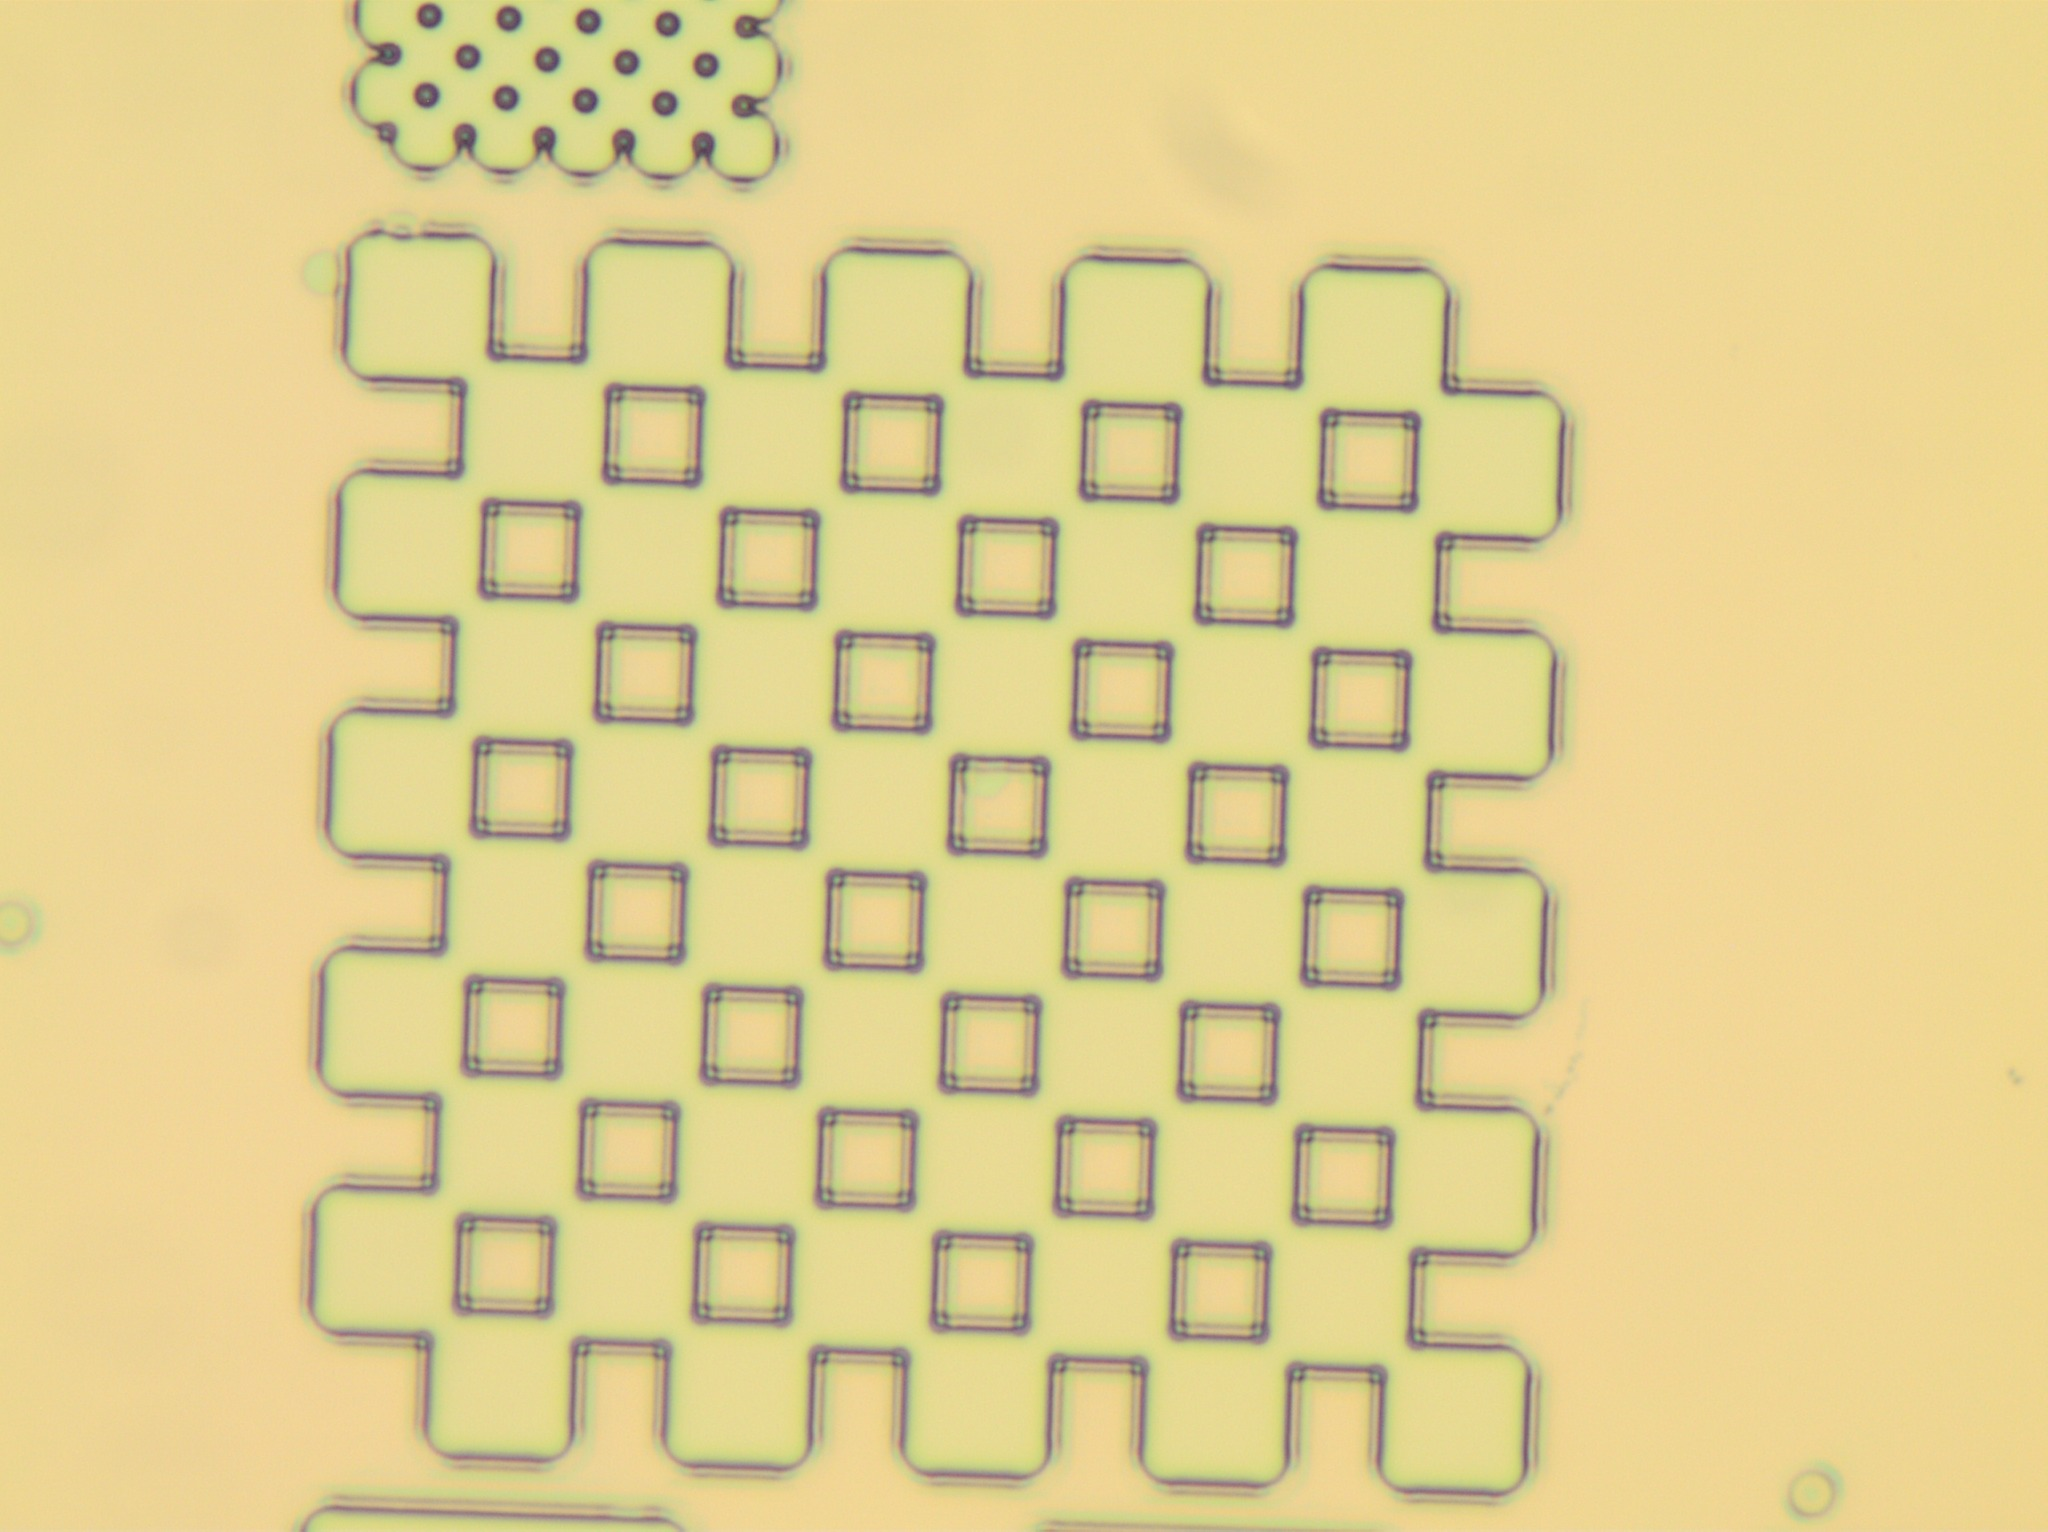
\includegraphics[width=\textwidth]{data/b3d1.jpg}
        \caption{One minute exposure. Significant underexposure is visible.}
        \label{fig:b3d1}
    \end{subfigure}
    \hfill
    \begin{subfigure}[t]{0.3\linewidth}
        \centering
        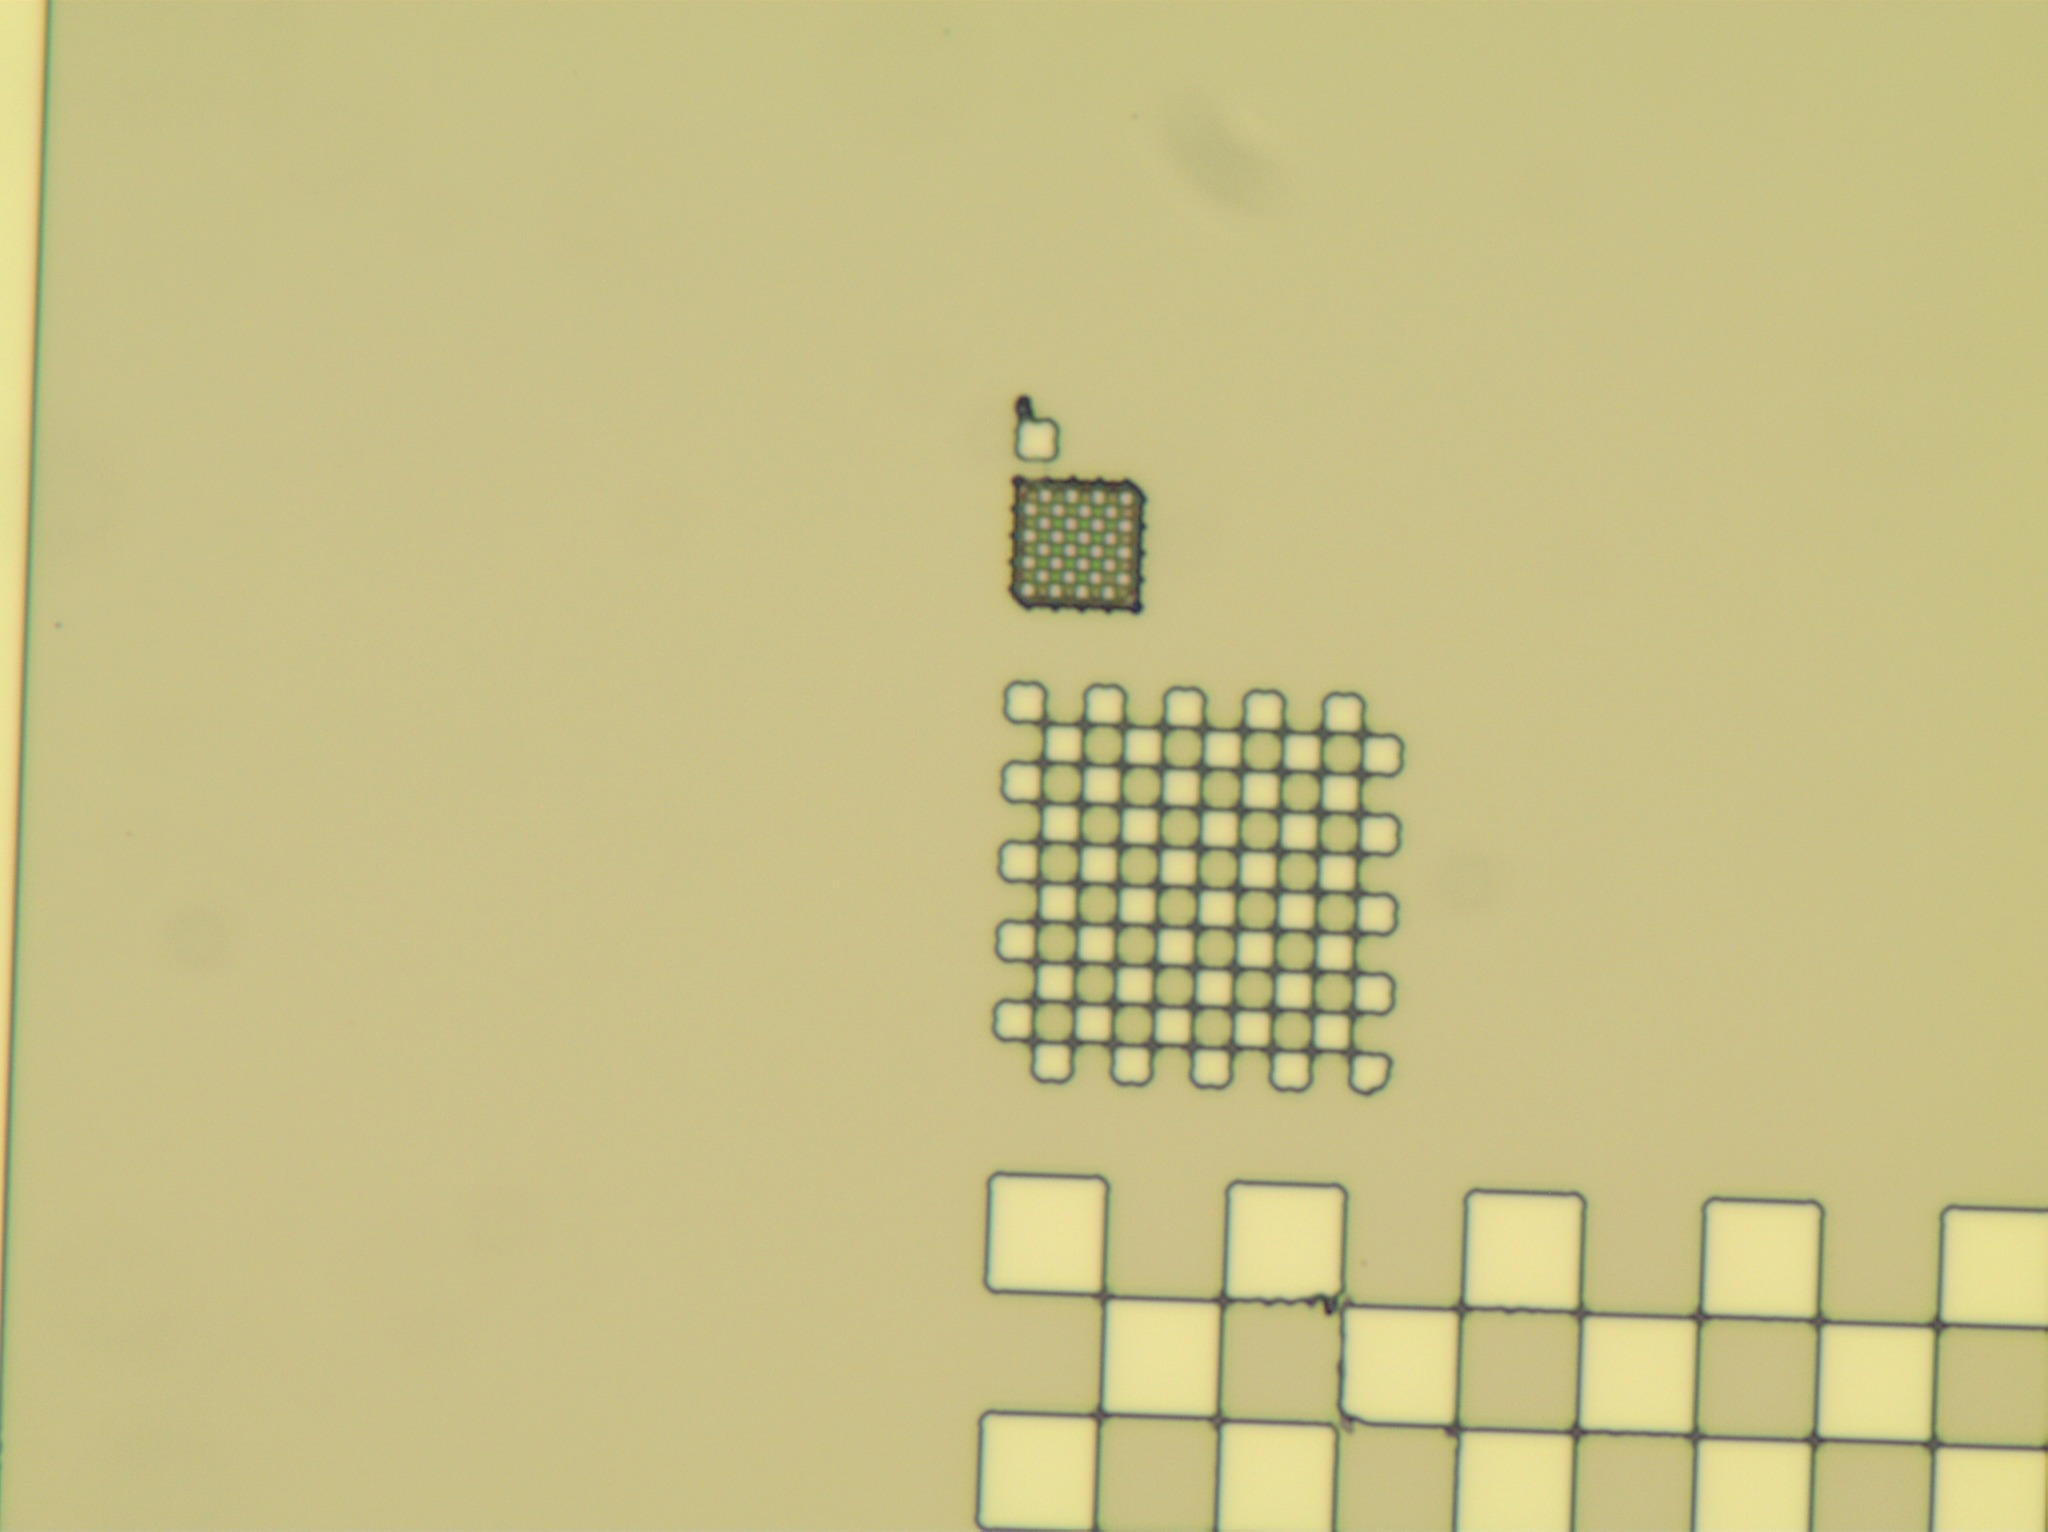
\includegraphics[width=\textwidth]{data/b3a1.jpg}
        \caption{Two minute exposure. The checkerboard pattern in the lower-right corner is of the same size as the one in figure \ref{fig:b2d1}.\todo[inline]{klopt de label?}}
        \label{fig:b3a1}
    \end{subfigure}
    \hfill
    \begin{subfigure}[t]{0.3\linewidth}
        \centering
        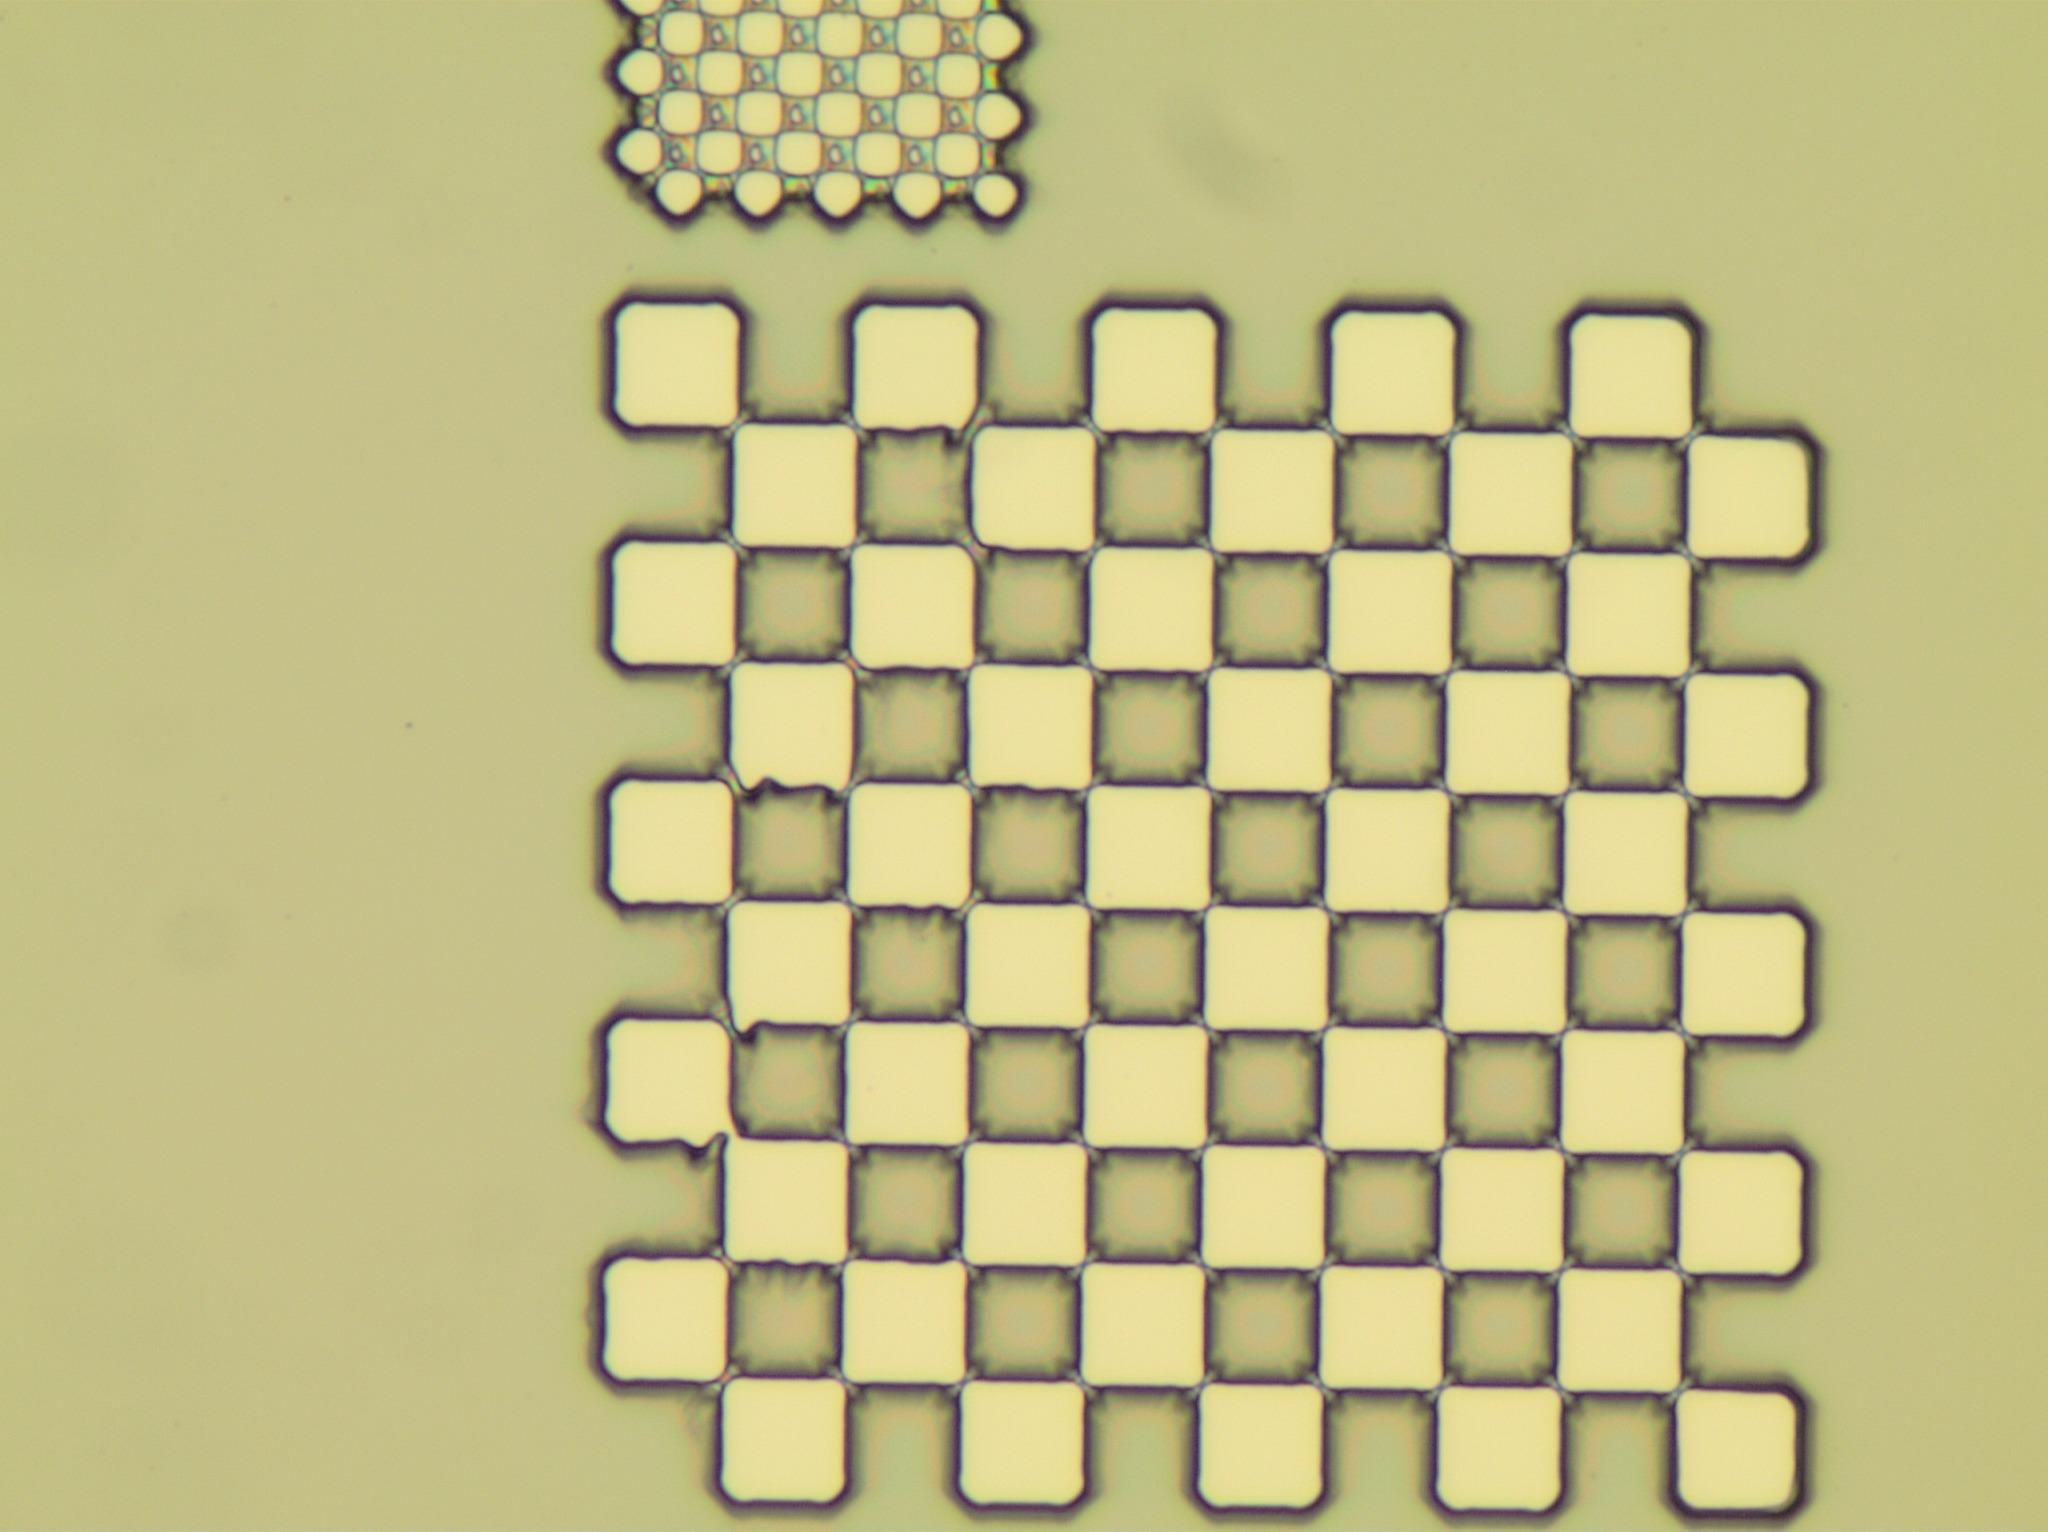
\includegraphics[width=\textwidth]{data/b3e1.jpg}
        \caption{2.5 minutes exposure. Slight overexposure at the vertices of the squares.}
        \label{fig:b3e1}
    \end{subfigure}
    \hfill
    % \rule{\linewidth}{3cm}
    \caption{Positive tone resist with different exposure times.}
\end{figure*}

\subsection*{Positive resist}
As a positive tone resist, AZ~5214E is used. To promote adhesion to the Si substrate, HMDS (hexamethyldisilazane) is applied first as a primer. The primer is deposited by hand on top of a silicon wafer and spun at 4000 RPM, it is then baked on a hot plate at 200$^{\circ}$~C for two minutes. The resist is spun at the same speed as the primer, which should result in a layer thickness of $1.40 \mu$m. The resist is baked on a hot plate at 90~$^{\circ}$C for one minute.

After the resist is deposited, the sample is exposed in the mask aligner for 1, 2, 2.5, 3, 3.5, and 4 minutes. After exposure the sample is developed for 60 seconds in MF-321 \footnote{MF-321 developer is mainly composed of water and tetramethylammonium hydroxide, it is produced by Microposit.} after which development is stopped by rinsing the sample another 60 seconds in purified water.

\subsection*{Negative resist}
AZ~5214E contains a special cross-linking agent which becomes active at temperatures above 110$^{\circ}$~C where the resist has been exposed. The cross-linking agent causes the individual molecules to bond, creating an almost insoluble, non-photoreactive substance. This allows the AZ~5214E to also be used as a negative resist.

Using the same mask as for the positive exposure, the sample is illuminated for a period of 0.1, 0.2, 0.3, 0.5, 1 and 1.5 minutes. After this first illumination the sample is baked in an oven at 120~$^\circ$C for 42 seconds. During this time cross-links are formed in the resist that was exposed during the first illumination. During baking the sample lies on an aluminium slab inside the oven, this prevents a large decrease in temperature when the oven door is opened and ensures good heat transfer to the sample. After baking, the entire sample is exposed (flood exposure) for a period of either 3 or 4 minutes. During this time the areas of the resist that are not cross-linked are cut up into smaller chains. When the sample is submerged in the MF-321 (again for 60 seconds), these smaller chains are dissolved. After development, the sample is rinsed with purified water as was done with the positive resist samples\cite{productdatasheet}.

